\section{Setup}


\begin{python}
import pennylane as qml
import numpy as np
import matplotlib.pyplot as plt
\end{python}

\begin{comment}
\begin{result}
\end{result}
\end{comment}

\newpage

\section{Following the paper}

\tcite{Frimmer_2014}.

\begin{center}
  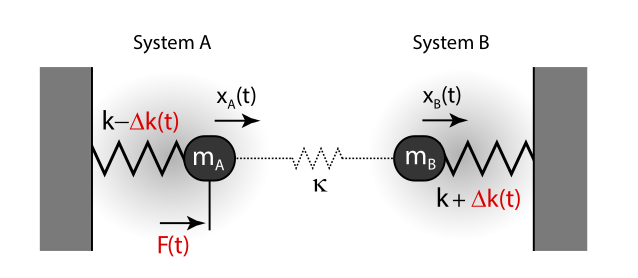
\includegraphics[width=0.6\textwidth]{img/osc.png}
\end{center}

The Newton's second law gives us the following equations:

\[
\begin{cases}
  \displaystyle F(t) - k \cdot x_a - \kappa(x_a - x_b) = m \ddot{x_a} \\
  \displaystyle \kappa(x_a - x_b) - k x_b = m \ddot{x_b}
\end{cases}
\]

The main motion equations are:

\[
\begin{cases}
  \displaystyle \ddot{x_a} + x_a\frac{k + \kappa}{m} - x_b\frac{\kappa}{m} = \frac{1}{m}F(t) \\
  \displaystyle \ddot{x_b} + x_b\frac{k + \kappa}{m} - x_a\frac{\kappa}{m} = 0
\end{cases}
\]

Following the paper, we define carrier frequency $\Omega_0^2 = \frac{k+\kappa}{m}$ and coupling
frequency $\Omega_c^2 = \frac{\kappa}{m}$.

\[
  m \frac{d^2x_A}{dt^2} + m \gamma \frac{dx_A}{dt} + \left(k + \kappa - \Delta
k(t)\right)x_A
  - \kappa x_B = F(t)
\]
\[
  m \frac{d^2x_B}{dt^2} + m \gamma \frac{dx_B}{dt} + \left(k + \kappa + \Delta
k(t)\right)x_B
  - \kappa x_A = 0
\]

Dividing by $m$.

\[
  \frac{d^2x_A}{dt^2} + \gamma \frac{dx_A}{dt} + \left(\frac{k + \kappa}{m} - \frac{\Delta
    k(t)}{m}\right)x_A -\frac{\kappa}{m}x_B = \frac{1}{m}F(t)
\]
\[
  \frac{d^2x_B}{dt^2} + \gamma \frac{dx_B}{dt} + \left(\frac{k + \kappa}{m} + \frac{\Delta
    k(t)}{m}\right)x_B -\frac{\kappa}{m}x_A = 0
\]

Introducing $\Omega$ frequencies:

\[
  \Omega_0^2 = [k + \kappa]/m
\]

\[
  \Omega_d^2 = \Delta k / m
\]

\[
  \Omega_c^2 = \kappa / m
\]

becomes

\[
\begin{pmatrix}
  \frac{d^2}{dt^2} + \gamma \frac{d}{dt} + \Omega_0^2
\end{pmatrix}
\begin{pmatrix}
 x_A \\
 x_B
\end{pmatrix}
+
\begin{pmatrix}
  -\Omega_d^2 & -\Omega_c^2 \\ -\Omega_c^2 & \Omega_d^2
\end{pmatrix}
\begin{pmatrix}
 x_A \\
 x_B
\end{pmatrix}
=
\begin{pmatrix}
 F(t) \\
 0
\end{pmatrix}
\]


\begin{ai}
Please rewrite the below two equation into the matrix form. I'd like to be like

\vsp

\verb|(...)(x_A ; x_B) + (...) (x_A; x_B) = (f(t) ; 0)|.

\[
  \frac{d^2x_A}{dt^2} + \gamma \frac{dx_A}{dt} + \left(\frac{k + \kappa}{m} - \frac{\Delta
    k(t)}{m}\right)x_A -\frac{k}{m}x_B = \frac{1}{m}F(t)
\]
\[
  \frac{d^2x_B}{dt^2} + \gamma \frac{dx_B}{dt} + \left(\frac{k + \kappa}{m} + \frac{\Delta
    k(t)}{m}\right)x_B -\frac{k}{m}x_A = 0
\]

Introducing $\Omega$ frequencies:

\[
  \Omega_0^2 = [k + \kappa]/m
\]

\[
  \Omega_d^2 = \Delta k / m
\]

\[
  \Omega_c^2 = \kappa / m
\]


\end{ai}

\begin{airesult}
To rewrite the given equations in matrix form, we'll utilize the newly introduced frequencies
\(\Omega_0\), \(\Omega_d\), and \(\Omega_c\). We then represent the system using matrix operations
on a vector composed of \(x_A\) and \(x_B\).

The two equations provided are:

\vsp

\[
\frac{d^2x_A}{dt^2} + \gamma\frac{dx_A}{dt} + \left( \frac{k + \kappa}{m} - \frac{\Delta k(t)}{m}
\right)x_A
- \frac{k}{m}x_B = \frac{1}{m}F(t)
\]

\[
\frac{d^2x_B}{dt^2} + \gamma\frac{dx_B}{dt} + \left( \frac{k + \kappa}{m} + \frac{\Delta k(t)}{m}
\right)x_B
- \frac{k}{m}x_A = 0
\]

\vsp

Using the new frequency parameters, the equations become:

\vsp

\[
\frac{d^2x_A}{dt^2} + \gamma\frac{dx_A}{dt} + \left( \Omega_0^2 - \Omega_d^2 \right)x_A
- \frac{k}{m}x_B = \frac{1}{m}F(t)
\]

\[
\frac{d^2x_B}{dt^2} + \gamma\frac{dx_B}{dt} + \left( \Omega_0^2 + \Omega_d^2 \right)x_B
- \frac{k}{m}x_A = 0
\]

\vsp

To express these in a matrix form:

\[
\begin{pmatrix}
 \frac{d^2}{dt^2} + \gamma \frac{d}{dt} + (\Omega_0^2 - \Omega_d^2) & -\frac{k}{m} \\
 -\frac{k}{m} & \frac{d^2}{dt^2} + \gamma \frac{d}{dt} + (\Omega_0^2 + \Omega_d^2)
\end{pmatrix}
\begin{pmatrix}
 x_A \\
 x_B
\end{pmatrix}
=
\begin{pmatrix}
 \frac{1}{m}F(t) \\
 0
\end{pmatrix}
\]

\vsp

This representation condenses the system of differential equations into a single matrix equation,
allowing easier manipulation and understanding of the coupled dynamics.
\end{airesult}


\section{Following the book}
\tcite{smith2010waves}.

\subsection{Coupled oscillators}

\[
\begin{aligned}
  \ddot{x}_1 + \frac{g}{\ell} x_1 + \frac{k}{m} (x_1 - x_2) &= 0, \\
  \ddot{x}_2 + \frac{g}{\ell} x_2 + \frac{k}{m} (x_2 - x_1) &= 0
\end{aligned}
\]


\begin{python}
import numpy as np
from scipy.integrate import solve_ivp
import matplotlib.pyplot as plt

# Constants
m = 0.1  # mass in kg
l = 0.15  # length in m
k = 0.5  # spring constant in N/m
g = 9.81  # acceleration due to gravity in m/s^2

# Initial conditions
def coupled_oscillators(name, x1_0 = 0.01, x2_0 = 0.01, v1_0 = 0.0, v2_0 = 0.0):
  '''
  x1_0 = 0.01  # initial position of x1 in m
  x2_0 = 0.01  # initial position of x2 in m
  v1_0 = 0.0  # initial velocity of x1
  v2_0 = 0.0  # initial velocity of x2
  '''

  # System of equations
  def _ode(t, y):
    x1, v1, x2, v2 = y
    dx1dt = v1
    dv1dt = -(g / l) * x1 - (k / m) * (x1 - x2)
    dx2dt = v2
    dv2dt = -(g / l) * x2 - (k / m) * (x2 - x1)
    return [dx1dt, dv1dt, dx2dt, dv2dt]

  # Time span for the simulation
  t_span = (0, 10)  # simulate from t=0 to t=10 seconds
  t_eval = np.linspace(t_span[0], t_span[1], 1000)  # time points to evaluate at

  # Initial state vector
  y0 = [x1_0, v1_0, x2_0, v2_0]

  # Solve the system of ODEs
  solution = solve_ivp(_ode, t_span, y0, t_eval=t_eval)

  # Plot the results on separate subplots
  plt.figure(figsize=(10, 8))

  # Plot for x1
  plt.subplot(211)
  plt.plot(solution.t, solution.y[0], label=r'$x_1$', color='b')
  plt.ylabel('Displacement (m)')
  plt.title('Coupled Oscillator Simulation')
  plt.legend(loc='upper right')
  plt.grid(True)

  # Plot for x2
  plt.subplot(212, sharex=plt.gca())
  plt.plot(solution.t, solution.y[2], label=r'$x_2$', color='r')
  plt.xlabel('Time (s)')
  plt.ylabel('Displacement (m)')
  plt.legend(loc='upper right')
  plt.grid(True)

  plt.tight_layout()
  plt.savefig(f"img/mechanical-bloch-f1-{name}.png")

coupled_oscillators("1", 0.01, 0.01)
coupled_oscillators("2", 0.01, -0.01)
coupled_oscillators("3", 0.01, 0)
\end{python}

\begin{comment}
\begin{result}
\end{result}
\end{comment}

\begin{figure}[H]
  \centering
  \includegraphics[width=0.4\linewidth]{img/mechanical-bloch-f1-1.png}
  \includegraphics[width=0.4\linewidth]{img/mechanical-bloch-f1-2.png}
  \includegraphics[width=0.4\linewidth]{img/mechanical-bloch-f1-3.png}
  \caption{(1) Pendulum normal mode (2) Breathing normal mode. The amplitudes are the same but we
  need more potential energy to run this mode to draw the spring. (3) Energy transmission from one
  oscillator to another via the connecting spring.}
  \label{fig:mechanical-bloch}
\end{figure}


\subsection{Discussion}

\subsubsection{Simulation}
\begin{ai}

Hi model. Please consider the below example file (Latex) describing a working simulation of the
Maxwell equation:

/append file:maxwell-sim.tex in

(end of example).

I have the following formulas describing a coupled oscillator:

\[
\begin{aligned}
  \ddot{x}_1 + \frac{g}{\ell} x_1 + \frac{k}{m} (x_1 - x_2) &= 0, \\
  \ddot{x}_2 + \frac{g}{\ell} x_2 + \frac{k}{m} (x_2 - x_1) &= 0
\end{aligned}
\]

Please generate me a code in Python which would simulate these formulas, given $m=0.1$ kg, $l=0.15
$ m, $k = 0.5$ N/m, At $t=0$, let both $x_1 = 1$ cm and $x_2 = 1$ cm.

\end{ai}

\begin{airesult}
To simulate the system of coupled oscillators described by the differential equations, we can use
numerical integration methods. One common approach is the \textit{Runge-Kutta method}, which is
well-suited for solving ordinary differential equations (ODEs). Here's a Python code example that
sets up and solves the system using the \verb|scipy| library's \verb|solve_ivp| function:

\begin{python}
import numpy as np
from scipy.integrate import solve_ivp
import matplotlib.pyplot as plt

# Constants
m = 0.1  # mass in kg
l = 0.15  # length in m
k = 0.5  # spring constant in N/m
g = 9.81  # acceleration due to gravity in m/s^2

# Initial conditions
x1_0 = 0.01  # initial position of x1 in m
x2_0 = 0.01  # initial position of x2 in m
v1_0 = 0.0  # initial velocity of x1
v2_0 = 0.0  # initial velocity of x2

# System of equations
def coupled_oscillators(t, y):
  x1, v1, x2, v2 = y
  dx1dt = v1
  dv1dt = -(g / l) * x1 - (k / m) * (x1 - x2)
  dx2dt = v2
  dv2dt = -(g / l) * x2 - (k / m) * (x2 - x1)
  return [dx1dt, dv1dt, dx2dt, dv2dt]

# Time span for the simulation
t_span = (0, 10)  # simulate from t=0 to t=10 seconds
t_eval = np.linspace(t_span[0], t_span[1], 1000)  # time points to evaluate at

# Initial state vector
y0 = [x1_0, v1_0, x2_0, v2_0]

# Solve the system of ODEs
solution = solve_ivp(coupled_oscillators, t_span, y0, t_eval=t_eval)

# Plot the results on separate subplots
plt.figure(figsize=(10, 8))

# Plot for x1
plt.subplot(211)
plt.plot(solution.t, solution.y[0], label=r'$x_1$', color='b')
plt.ylabel('Displacement (m)')
plt.title('Coupled Oscillator Simulation')
plt.legend(loc='upper right')
plt.grid(True)

# Plot for x2
plt.subplot(212, sharex=plt.gca())
plt.plot(solution.t, solution.y[2], label=r'$x_2$', color='r')
plt.xlabel('Time (s)')
plt.ylabel('Displacement (m)')
plt.legend(loc='upper right')
plt.grid(True)

plt.tight_layout()
plt.show()
\end{python}

The code sets up the system of differential equations for the coupled oscillators based on the
provided formulas. It defines initial conditions for \(x_1\) and \(x_2\) as \(1 \ \text{cm} = 0.01 \
\text{m}\), and uses the \verb|solve_ivp| function from \verb|scipy.integrate| to perform the
integration over the specified time span. The results are then plotted using \verb|matplotlib| to
visualize the displacement over time for both oscillators.
\end{airesult}

\subsubsection{Runge-Kutta}

\begin{ai}
Please tell me more about Runge-Kutta method. What kind of DE can it solve?
\end{ai}

\begin{airesult}
The Runge-Kutta methods are a family of iterative methods used for approximating solutions to
ordinary differential equations (ODEs). They are known for their accuracy and efficiency, making
them a popular choice for solving a wide range of ODEs, particularly when analytical solutions are
challenging or impossible to obtain.

\vsp

Here are some key aspects of the Runge-Kutta methods:

\begin{itemize}
\item \textbf{Types of Equations:}

  \begin{itemize}
  \item Runge-Kutta methods are primarily used for first-order ODEs of the form:
  \[
  \frac{dy}{dt} = f(t, y)
  \]
  where \(y\) is the dependent variable, \(t\) is the independent variable, and \(f\) is a function
that describes the system.

  \item Higher-order ODEs can be solved by converting them into a system of first-order ODEs. For
example, a second-order ODE can be rewritten using two first-order ODEs by introducing auxiliary
variables for each derivative.

  \end{itemize}

\item \textbf{The Classical Fourth-Order Runge-Kutta Method (RK4):}

  \begin{itemize}
  \item The RK4 method is a popular version that provides a good balance between accuracy and
computational cost. It estimates the solution by taking the weighted average of slopes (derivatives)
at several points within the integration step.

  \item The RK4 algorithm involves four intermediate calculations, known as \textit{stages}, per
time step to approximate the next value:

  \[
  \begin{aligned}
  k_1 &= f(t_n, y_n), \\
  k_2 &= f\left(t_n + \frac{\Delta t}{2}, y_n + \frac{k_1 \Delta t}{2}\right), \\
  k_3 &= f\left(t_n + \frac{\Delta t}{2}, y_n + \frac{k_2 \Delta t}{2}\right), \\
  k_4 &= f(t_n + \Delta t, y_n + k_3 \Delta t),
  \end{aligned}
  \]

  \item The next value of \( y \) is then found by:

  \[
  y_{n+1} = y_n + \frac{\Delta t}{6} (k_1 + 2k_2 + 2k_3 + k_4)
  \]

  \end{itemize}

\item \textbf{Applications:}

  \begin{itemize}
  \item Runge-Kutta methods can be used to solve a vast range of problems, including systems
modeling physical phenomena (e.g., mechanics, orbital dynamics), biological processes, electrical
circuits, and any situation well-modeled by ODEs.
  \item They can handle various initial value problems and are appropriate for stiff and non-stiff
ODEs when carefully chosen. However, for very stiff equations, specialized methods (like implicit
Runge-Kutta methods) might be more suitable.
  \end{itemize}

\item \textbf{Advantages and Limitations:}

  \begin{itemize}
  \item Runge-Kutta methods are straightforward to implement, versatile, and capable of high
precision.
  \item They are computationally intensive compared to simpler methods like Euler's method, but
generally offer better stability and accuracy.
  \item They require careful step-size control; adaptive step-size versions of the Runge-Kutta
methods can be used to achieve better efficiency and accuracy.
  \end{itemize}

\end{itemize}

\vsp

The Runge-Kutta methods, with RK4 being the most widely implemented, are robust tools for
numerically solving a broad class of ODEs encountered in scientific computing, engineering, and
physics.
\end{airesult}


\subsubsection{Runge-Kutta vs FDTD}

\begin{ai}
Can you compare Runge-Kutta with FDTD method?
\end{ai}

\begin{airesult}
Certainly! Both the Runge-Kutta and Finite-Difference Time-Domain (FDTD) methods are numerical
techniques used for solving differential equations, but they are employed in different contexts and
have distinct characteristics. Let's compare them:

\vsp

\begin{itemize}
\item \textbf{Purpose and Application:}

  \begin{itemize}
  \item \textbf{Runge-Kutta (RK) Methods:}
    - Primarily designed for solving ordinary differential equations (ODEs).
    - Widely used in a variety of fields, such as engineering, physics, and other sciences, for
problems involving time-dependent systems or dynamics.
    - A versatile choice for systems where the equations involve one independent variable, often
time.

  \item \textbf{Finite-Difference Time-Domain (FDTD) Method:}
    - Specifically developed for solving Maxwell's equations in the time-domain to model
electromagnetic wave propagation.
    - Commonly applied in computational electromagnetics for simulating fields around antennas,
waveguides, and other RF/microwave structures.
    - Suitable for partial differential equations (PDEs) involving both spatial and time dimensions.

  \end{itemize}

\item \textbf{Algorithm and Technique:}

  \begin{itemize}
  \item \textbf{Runge-Kutta Methods:}
    - Use multiple stages (e.g., 4 stages in RK4) to improve accuracy by estimating the solution's
slope at various points within each time step.
    - Considered explicit methods; they work step-by-step using initial conditions without needing
to solve simultaneous equations at each time step.

  \item \textbf{FDTD Method:}
    - Based on discretizing both space and time using finite differences, approximating derivatives
with differences.
    - Applies both explicit and sometimes implicit techniques to update field values in a grid
iteratively.
    - Used extensively in grid-based simulations of wave interactions where spatial-temporal
accuracy is essential.

  \end{itemize}

\item \textbf{Strengths and Use Cases:}

  \begin{itemize}
  \item \textbf{Runge-Kutta Methods:}
    - High precision for well-posed initial value problems in ODEs.
    - Preferred for non-stiff and moderately stiff systems with complex dynamics.
    - Adaptive step-size versions allow efficient computation.

  \item \textbf{FDTD Method:}
    - Excellent for capturing wave phenomena and field interactions in heterogeneous media.
    - Direct simulation of wave reflections, diffraction, interference, and scattering.
    - Highly parallelizable; often implemented in parallel computing frameworks.

  \end{itemize}

\item \textbf{Limitations:}

  \begin{itemize}
  \item \textbf{Runge-Kutta Methods:}
    - Only suitable for ordinary differential equations (one independent variable).
    - Can be computationally intensive for very stiff systems.

  \item \textbf{FDTD Method:}
    - Computationally demanding, requiring fine spatial and temporal discretization to maintain
accuracy.
    - Requires careful handling of boundary conditions to prevent artificial reflections.

  \end{itemize}

\end{itemize}

\vsp

In essence, while both Runge-Kutta and FDTD methods aim to numerically solve differential equations,
they cater to different types of problems. The Runge-Kutta method is a general-purpose tool for
ODEs, whereas FDTD is specialized for simulating electromagnetic fields and wave interactions
governed by Maxwell's equations.
\end{airesult}

\subsubsection{ODE}

\begin{ai}
OK, now please define ordinary DE. What is dependant variable? Why is it different from a function?
\end{ai}

\begin{airesult}
An ordinary differential equation (ODE) is a type of differential equation involving functions of a
single independent variable and their derivatives. ODEs describe the rate of change of a dependent
variable with respect to an independent variable. Here is a more detailed explanation:

\vsp

\begin{itemize}
\item \textbf{Definition of ODE:}

  \begin{itemize}
  \item An ODE can be written in its general form as:
  \[
  F\left(t, y, \frac{dy}{dt}, \frac{d^2y}{dt^2}, \ldots, \frac{d^n y}{dt^n}\right) = 0
  \]
  where \(y\) is a dependent variable, \(t\) is the independent variable, and \(F\) is a function
representing the relationship between these variables and their derivatives.

  \item The order of an ODE is determined by the highest derivative of the dependent variable
present in the equation. For example, a first-order ODE involves only the first derivative
\(\frac{dy}{dt}\).

  \item ODEs are classified into linear and nonlinear equations based on the degree of the dependent
variable and its derivatives. Linear ODEs have the dependent variable and its derivatives to the
power of one, without multiplication between them.

  \end{itemize}

\item \textbf{Dependent Variable:}

  \begin{itemize}
  \item The dependent variable (\(y\) in our example) is the quantity whose variations we are
interested in studying. It is typically a function of the independent variable.

  \item In the context of an ODE, the dependent variable represents the unknown whose behavior is
described by the differential equation. It changes in response to changes in the independent
variable.

  \item The solution to an ODE is a function \( y(t) \) describing how the dependent variable
evolves over the domain of the independent variable.

  \end{itemize}

\item \textbf{Difference from a Function:}

  \begin{itemize}
  \item While the dependent variable is a specific variable being solved for in an ODE, a function
is a broader mathematical concept representing a relationship between variables, typically defined
by an explicit formula or rule.

  \item In an ODE, \( y(t) \) is the function that serves as the solution, expressing the dependent
variable in terms of the independent variable. It describes the behavior or state of the dependent
variable over time or space.

  \item The outcome of solving an ODE is the function itself, which reveals how the dependent
variable changes, providing insights into the underlying dynamic system.

  \end{itemize}

\end{itemize}

\vsp

In summary, ODEs play a crucial role in modeling a wide array of real-world phenomena where a single
independent variable influences the behavior of another variable, such as time-dependent processes
in physics, engineering, and beyond.
\end{airesult}
